\documentclass[11pt]{article}

% ---------- packages ----------
\usepackage[margin=1in]{geometry}
\usepackage{amsmath,amssymb,mathtools}
\usepackage{booktabs}
\usepackage{array}
\usepackage{enumitem}
\usepackage{xcolor}
\usepackage{listings}
\usepackage{hyperref}
\usepackage{tikz}
\usetikzlibrary{arrows.meta, positioning, fit, backgrounds}

% ---------- code listing style ----------
\definecolor{codebg}{RGB}{245,245,245}
\definecolor{codekw}{RGB}{0,90,180}
\lstset{
  language=JavaScript,
  basicstyle=\ttfamily\small,
  keywordstyle=\color{codekw}\bfseries,
  commentstyle=\color{gray}\itshape,
  numbers=none,
  backgroundcolor=\color{codebg},
  frame=single,
  rulecolor=\color{gray!40},
  breaklines=true,
  showstringspaces=false,
  tabsize=2,
  xleftmargin=1em,
  xrightmargin=1em
}

% ---------- tikz styles ----------
\tikzset{
  block/.style={rectangle, draw=black!70, rounded corners, fill=blue!7,
    text width=6.4cm, align=center, minimum height=1.05cm, font=\small},
  data/.style={rectangle, draw=black!60, fill=yellow!12,
    text width=5.6cm, align=center, minimum height=0.9cm, font=\small\ttfamily},
  gpu/.style={rectangle, draw=black!70, thick, fill=green!8,
    text width=6.4cm, align=center, minimum height=1.05cm, font=\small},
  arrowline/.style={-{Latex[length=2.2mm]}, thick},
}

% ---------- convenience macros ----------
\newcommand{\code}[1]{\texttt{#1}}
\newcommand{\func}[1]{\texttt{\textbf{#1}}}
\newcommand{\type}[1]{\textsc{#1}}
\newcommand{\R}{\mathbb{R}}

\title{\textbf{heat-flow.ts, Frame by Frame}\\[2pt]
\large From the geodesic distance field $\varphi$ to a pixel on screen}
\author{projects/heat-flow/heat-flow.ts}
\date{}

\begin{document}
\maketitle

\begin{center}
\begin{minipage}{0.9\textwidth}
\small
\textbf{Scope.} \code{notes/heat-method-blueprint.tex} already derives how
\code{heatMethod.compute(delta)} produces $\varphi$ (\code{phi}), the per-vertex geodesic
distance from a clicked source. This document starts exactly there --- $\varphi$ is a
given input --- and traces everything downstream of it: every variable that gets
introduced, every TSL function the shader graph is built from, and, since this script
\emph{animates}, precisely what changes from one rendered frame to the next and what stays
fixed. The current version of the shader (``V2 Wavefront'') renders a single narrow
\emph{band} that travels outward through $\varphi$-space and back out again --- not a
filled region that grows and stays filled --- so a vertex flares through a color ramp and
then returns to its resting color as the band passes over it. Two independent ``loops''
are involved and this document is organized around that split:
\begin{itemize}[leftmargin=1.4em]
  \item \textbf{The one-shot pipeline} (\func{diffuseFrom}) --- runs once, synchronously,
    every time the user taps a new source vertex. It is plain CPU/JavaScript code.
  \item \textbf{The per-frame pipeline} (\func{animateWave}, called from
    \func{engine.run}'s callback, plus the already-compiled GPU shader) --- runs
    continuously, roughly 60 times a second, whether or not anything has been clicked.
\end{itemize}
The one-shot pipeline sets up everything the per-frame pipeline needs; the per-frame
pipeline then advances exactly \emph{one} number (\code{waveProgress.value}) every tick and
lets the GPU redraw the whole mesh from that, combined with the \code{waveMaxDistance}
uniform it set once at click time.
\end{minipage}
\end{center}

\tableofcontents

% =====================================================================
\section{The input: \texorpdfstring{$\varphi$}{phi}}
\label{sec:input}
% =====================================================================

\code{heatMethod.compute(delta)} (Section~2 of \code{heat-method-blueprint.tex}) returns
\code{phi} : \type{DenseMatrix} of shape $V\times1$ --- one non-negative real number
$\varphi_i \ge 0$ per mesh vertex $i$, the approximate geodesic distance from vertex $i$ to
whichever vertex was clicked, measured in the mesh's own normalized units (the mesh is
rescaled to fit a unit ball by \code{loadObjAsset}, so $\varphi$'s scale is tied to that,
not to any real-world unit). Everything in this document is about what happens to those
numbers \emph{after} they come out of \code{compute()} --- getting them onto the GPU, and
turning them into a color that changes convincingly over time.

% =====================================================================
\section{Variable inventory}
\label{sec:vars}
% =====================================================================

Every variable in the file, grouped by \emph{how long it lives} and \emph{who changes it}
--- this grouping is the single most useful lens for answering ``what changes over time.''

\begin{center}
\small
\renewcommand{\arraystretch}{1.35}
\begin{tabular}{@{}p{2.6cm}p{2.6cm}p{9cm}@{}}
\toprule
\textbf{Variable} & \textbf{Lifetime} & \textbf{What it is / why it exists} \\
\midrule
\code{CYAN}, \code{MAGENTA} & module constant & Hex RGB integers left over from the
  previous (``V1 Spread'') version of this shader. Still defined, but \textbf{no longer
  read anywhere} in the current shader graph --- dead code since the rewrite to a
  traveling band. \\
\code{BASE\_COLOR} & module constant & \code{color(0x00e5ff)} --- the same cyan as the old
  \code{CYAN}, but wrapped as a TSL color node and actually used: it's the resting color a
  vertex sits at before/after the wave passes over it. \\
\code{FIRE\_COLOR\_1}, \code{FIRE\_COLOR\_2}, \code{FIRE\_COLOR\_3} & module constant &
  Red, yellow, and white --- the three stops of the color ramp a vertex sweeps through as
  wave intensity rises from $0$ to $1$ (Section~\ref{sec:shader}). \\
\code{WAVE\_DURATION} & module constant & $5$ --- real-world seconds the band takes to
  cross the entire span from just-behind-the-source to just-past-the-farthest-vertex.
  Never changes. \\
\code{TAP\_THRESHOLD\_PX} & module constant & $6$ --- pointer-movement threshold (pixels)
  distinguishing a tap (pick a vertex) from a drag (orbit the camera). Unrelated to color;
  listed for completeness. \\
\midrule
\code{vertexCount} & set once, in \func{init()} & $V$, the mesh's vertex count. Read-only
  afterward. \\
\code{distances} & set once (the array), \emph{contents} overwritten every click &
  \type{Float32Array} of length $V$ --- the CPU-side mirror of $\varphi$ that actually
  backs the GPU buffer. Starts filled with $0.0$ everywhere (unlike the old V1 version,
  which started at a large sentinel value; see Section~\ref{sec:timeline} for why $0.0$
  still reads as ``untouched'' here). \\
\code{distanceAttribute} & set once & \type{THREE.BufferAttribute} wrapping \code{distances}
  and attached to the mesh's geometry under the name \code{"geodesicDist"} (renamed from
  the old \code{"heatDistance"}) --- see Section~\ref{sec:oneshot}. \\
\code{waveProgress}, \code{waveMaxDistance} & set once (as \type{UniformNode}s) &
  Returned by \func{createHeatFlowMaterial()} (Section~\ref{sec:shader}); both are TSL
  uniforms whose \code{.value} fields are the only things the CPU-side code touches after
  creation --- \code{waveProgress} every frame, \code{waveMaxDistance} once per click. \\
\code{waveGlowNode} & set once & Also returned by \func{createHeatFlowMaterial()} --- a
  \func{Fn(...)}-wrapped node-graph builder (Section~\ref{sec:shader}). \func{init()} calls
  it once, immediately, and assigns the result to \code{material.colorNode}. \\
\code{material} & set once, in \func{init()} & A \type{THREE.MeshStandardNodeMaterial};
  unlike the old V1 version, building the material itself is no longer
  \func{createHeatFlowMaterial()}'s job --- that function only builds the uniforms and the
  color node graph, and \func{init()} does the \code{new THREE.MeshStandardNodeMaterial()}
  plus the \code{colorNode}/\code{roughnessNode}/\code{metalnessNode} assignments itself. \\
\midrule
\code{sendWave} & toggled by clicks and by \func{animateWave} & Boolean. Set \code{true} by
  the \emph{first} click after being idle; set back to \code{false} by
  \func{animateWave} once \code{progress} reaches $1$. Gates whether
  \func{animateWave} does anything at all. \\
\code{animationStartTime} & conditionally overwritten by clicks & \code{performance.now()}
  at the instant a wave \emph{starts} being sent. Critically, this is only reset when
  \code{sendWave} was \code{false} at click time --- see the quirk called out in
  Section~\ref{sec:oneshot}. \\
\midrule
\code{currentTime}, \code{elapsed}, \code{progress} & recomputed every frame inside
  \func{animateWave}, discarded immediately & \code{progress} is
  $\min(\text{elapsed}/\text{WAVE\_DURATION},\,1)$ --- a plain unitless $0\to1$ fraction of
  how far through the current wave's duration playback is. \\
\code{waveProgress.value} & \textbf{the one thing written every frame} (while a wave is
  active) & A plain JS number in $[0,1]$, copied into a tiny GPU-side uniform buffer; see
  Section~\ref{sec:perframe}. Notably, \emph{unlike} the old V1 version, this value is never
  multiplied by a distance on the CPU --- combining it with \code{waveMaxDistance} to get an
  actual $\varphi$-space position now happens inside the shader itself
  (Section~\ref{sec:shader}). \\
\bottomrule
\end{tabular}
\end{center}

% =====================================================================
\section{The one-shot pipeline: \func{diffuseFrom(vertexIndex)}}
\label{sec:oneshot}
% =====================================================================

Fires exactly once per tap, from the \code{pointerup} handler (via
\func{pickSourceVertex}, which is unrelated to color --- it just raycasts the click into
\code{threeMesh} and returns the nearest triangle-corner vertex index; see the file's own
comments for that part).

\begin{lstlisting}
function diffuseFrom(vertexIndex) {
  const delta = DenseMatrix.zeros(vertexCount, 1);
  delta.set(1, vertexIndex, 0);
  const phi = heatMethod.compute(delta);

  let maxDistance = 0;
  for (let i = 0; i < vertexCount; i++) {
    const d = phi.get(i, 0);
    distances[i] = d;
    if (d > maxDistance) maxDistance = d;
  }
  waveMaxDistance.value = maxDistance;
  waveProgress.value = 0.0;
  distanceAttribute.needsUpdate = true;

  if (!sendWave) {
    sendWave = true;
    animationStartTime = performance.now();
  }

  memoryManager.deleteExcept([heatMethod.A, heatMethod.F]);
}
\end{lstlisting}

\begin{enumerate}[leftmargin=1.6em]
\item \textbf{Solve.} \code{delta}/\code{phi} --- exactly the Goal~A pipeline from
  \code{heat-method-blueprint.tex}, treated here as a black box: one $V\times1$ vector in,
  one $V\times1$ vector ($\varphi$) out.
\item \textbf{Copy into a plain typed array, and find the maximum.} \code{phi} is a
  \type{DenseMatrix} --- a JS wrapper around memory that actually lives on the Emscripten/WASM
  heap (see the other blueprint's memory-management notes). A GPU buffer attribute needs a
  plain, contiguous \type{Float32Array} it can upload byte-for-byte; this loop is a single
  linear pass copying $\varphi_i \to \code{distances[i]}$ while simultaneously computing
  $\code{maxDistance} = \max_i \varphi_i$ --- no separate pass is needed for the max since
  it's cheap to track alongside the copy.
\item \textbf{Write both shader uniforms directly.} Unlike the old V1 version, which kept
  the ``how far this click has to travel'' number (\code{waveTarget}) as a plain JS
  variable and only pushed it into a single uniform's math on the CPU, this version writes
  \code{waveMaxDistance.value} straight from the solve, and always resets
  \code{waveProgress.value} to $0.0$ here too.
\item \textbf{Flag the buffer dirty.} \code{distanceAttribute.needsUpdate = true} is a
  three.js convention: a \type{BufferAttribute}'s CPU-side array can be freely mutated in
  place (as step 2 above just did), but the renderer only re-uploads it to the GPU on the
  \emph{next} frame if this flag is set --- otherwise, for performance, it assumes nothing
  changed and skips the upload entirely.
\item \textbf{Start the clock --- but only if idle.} This is the one genuinely subtle piece
  of behavior in this file. \code{animationStartTime} is \emph{only} reset when
  \code{sendWave} was \code{false} --- i.e.\ only on the first click after the previous wave
  finished (or at page load). If a second click lands \emph{while a wave is still in
  flight} (\code{sendWave} already \code{true}), this branch is skipped entirely:
  \code{animationStartTime} keeps its old value. The explicit
  \code{waveProgress.value = 0.0} write from step 3 still happens, but it is immediately
  overwritten on the very next rendered frame by \func{animateWave}
  (Section~\ref{sec:perframe}), which recomputes \code{progress} from the \emph{unchanged}
  \code{animationStartTime}. Practically: re-clicking mid-wave updates \emph{where} the
  band is centered relative to (the new \code{geodesicDist} field and
  \code{waveMaxDistance}) but does \emph{not} restart the sweep visually from the
  beginning --- the band can appear to jump straight to wherever the old timer's progress
  fraction already was. This is a real difference from the old V1 version, which
  unconditionally reset its timer on \emph{every} click. See
  Section~\ref{sec:timeline}'s last row for this played out concretely.
\item \textbf{Free WASM memory.} Exactly the cleanup call from the original blueprint's
  Section~4 --- \code{delta}, \code{phi}, and the Cholesky factorizations \code{compute()}
  allocated internally are all safe to free now, since step 2 already extracted every
  number this script needs from \code{phi} into a plain array.
\end{enumerate}

Nothing in this function runs more than once per click. In particular, \textbf{the shader
itself is never touched here} --- only uniform \code{.value}s and the attribute's backing
array are written; the compiled shader program doesn't change shape.

% =====================================================================
\section{The static shader graph: \func{createHeatFlowMaterial()}}
\label{sec:shader}
% =====================================================================

This function runs exactly \emph{once}, at page load, before any click has happened. It
builds a \emph{description} of a computation (a graph of small objects called
\type{Node}s) rather than performing the computation itself; three.js compiles that
description into a real GPU shader program (WGSL for the WebGPU backend, GLSL as a WebGL2
fallback) the first time the mesh is actually drawn, and the compiled program is what
runs, unchanged, on every frame afterward --- for every vertex and every on-screen pixel of
the mesh, in parallel, on the GPU. TSL (Three.js Shading Language) is exactly this: writing
shaders as composed JavaScript objects instead of a hand-written shader-language string.

\begin{lstlisting}
function createHeatFlowMaterial() {
  const waveProgress = uniform(0.0);
  const waveMaxDistance = uniform(1.0);
  const WAVE_LENGTH = 0.1;
  const startPos = -WAVE_LENGTH / 2;

  const waveGlowNode = Fn(() => {
    const endPos = waveMaxDistance.add(WAVE_LENGTH / 2);
    const waveCenter = waveProgress.mul(endPos.sub(startPos)).add(startPos);

    const vertexGeodesicDistance = attribute('geodesicDist', 'float');
    const distance = vertexGeodesicDistance.sub(waveCenter);

    const normalizedDistance = distance.div(WAVE_LENGTH / 2);
    const waveIntensity = cos(normalizedDistance.mul(Math.PI)).add(1.0).div(2.0);

    const isInsideWave = abs(normalizedDistance).lessThan(1.0);
    const finalIntensity = isInsideWave.select(waveIntensity, 0.0);

    const clippedIntensity = clamp(finalIntensity, 0.0, 1.0)
      .mul(waveProgress.lessThan(1.0).select(1.0, 0.0));

    const i3 = clippedIntensity.mul(3.0);
    const color_0_to_1 = mix(BASE_COLOR, FIRE_COLOR_1, i3);
    const color_1_to_2 = mix(FIRE_COLOR_1, FIRE_COLOR_2, i3.sub(1.0));
    const color_2_to_3 = mix(FIRE_COLOR_2, FIRE_COLOR_3, i3.sub(2.0));

    const finalColor = i3.lessThan(1.0).select(
      color_0_to_1,
      i3.lessThan(2.0).select(color_1_to_2, color_2_to_3)
    );

    return finalColor;
  });

  return { waveProgress, waveMaxDistance, waveGlowNode };
}
\end{lstlisting}

\subsection*{\func{Fn(() => \{...\})}}
\func{Fn} wraps a JS closure as a single compiled, reusable node --- the TSL equivalent of
writing a named function in a shader language, rather than an inline expression. Everything
inside the closure still just builds a graph (nothing executes yet); wrapping it in
\code{Fn} is what lets three.js compile the whole body as one unit and lets the caller treat
it as a single callable node factory (\code{waveGlowNode()}). This is the same pattern
\code{cube.js} uses for its reusable fresnel helper --- see that file for another example
of the same idiom.

\subsection*{\func{uniform(0.0)}, \func{uniform(1.0)}}
A \emph{uniform} is a GPU-programming term for a single value broadcast identically to
every invocation of a shader (as opposed to an \emph{attribute}, below, which differs per
vertex). \code{uniform(x)} returns a \type{UniformNode} wrapping the JS number \code{x},
and critically, its \code{.value} property is a \emph{live} hook: writing
\code{waveProgress.value = 0.83} from ordinary JavaScript updates a small piece of GPU
memory (a uniform buffer) that the \emph{already-compiled} shader reads on its very next
invocation --- no recompilation, no rebuilding this node graph. This is the entire
mechanism the per-frame pipeline (Section~\ref{sec:perframe}) relies on to animate anything
at all cheaply, 60 times a second. This shader now reads \emph{two} independent uniforms
--- \code{waveProgress} (rewritten every frame) and \code{waveMaxDistance} (rewritten once
per click) --- rather than the single \code{waveRadius} the old V1 version used.

\subsection*{\code{waveCenter}: the band's travel math}
\[
  \text{endPos} = \text{waveMaxDistance} + \tfrac{\text{WAVE\_LENGTH}}{2}, \qquad
  \text{startPos} = -\tfrac{\text{WAVE\_LENGTH}}{2}
\]
\[
  \text{waveCenter}(\text{waveProgress}) = \text{waveProgress}\cdot(\text{endPos}-\text{startPos}) + \text{startPos}
\]
This is a plain linear interpolation from \code{startPos} to \code{endPos} as
\code{waveProgress} runs $0\to1$. The endpoints are chosen so the band's \emph{center}
starts \emph{behind} the source (at $-\text{WAVE\_LENGTH}/2$, i.e.\ half a band-width before
$\varphi=0$) and finishes \emph{past} the farthest vertex (at
$\text{waveMaxDistance}+\text{WAVE\_LENGTH}/2$) --- so both the closest and farthest
vertices get a smooth ramp-in / ramp-out instead of the band snapping to full intensity the
instant it reaches them. Note this is exactly the unit-conversion step the old V1 version
did on the CPU (multiplying \code{progress} by \code{waveTarget} before ever touching the
GPU); here it happens on the GPU instead, every fragment, every frame, from the two raw
uniforms.

\subsection*{\func{attribute('geodesicDist', 'float')}}
An \emph{attribute} is the GPU-programming term for a per-vertex input --- \code{position}
and \code{normal} are attributes too, just ones three.js wires up automatically.
\code{'geodesicDist'} is a \emph{custom} attribute this script defined itself
(\code{threeMesh.geometry.setAttribute('geodesicDist', distanceAttribute)},
Section~\ref{sec:oneshot}); \code{attribute(name, type)} is TSL's way of saying ``read this
named per-vertex buffer, as this GLSL/WGSL type, wherever the graph ends up needing it.''

As before, the detail that actually explains why the mesh looks smoothly shaded rather than
faceted: \code{geodesicDist} is fed into \code{colorNode}, and color must be computed once
per \emph{fragment} (i.e.\ once per on-screen pixel a triangle covers), not merely once per
vertex. Whenever an attribute node like this is consumed somewhere that needs a
per-fragment value, TSL automatically inserts a \emph{varying}: the GPU computes
$\varphi$ at each of a triangle's three vertices (three numbers), and the rasterizer
hardware then linearly interpolates between those three values, per pixel, using
barycentric weights, entirely for free. So the raw data really is coarse --- one number per
vertex --- but nothing downstream of it (the wave-intensity math, the color ramp) ever sees
a hard per-triangle jump; it sees a continuously-varying value across every pixel.

\subsection*{\func{normalizedDistance} and \func{cos(...)}: the raised-cosine band}
\[
  \text{normalizedDistance} = \frac{\varphi_i - \text{waveCenter}}{\text{WAVE\_LENGTH}/2},
  \qquad
  \text{waveIntensity} = \frac{\cos(\pi \cdot \text{normalizedDistance}) + 1}{2}
\]
\code{normalizedDistance} rescales a fragment's distance from the band's center into units
where $\pm1$ is exactly the band's edge. \code{cos} is a standard GLSL/WGSL built-in
trigonometric function; the expression $(\cos(\pi t)+1)/2$ is a \emph{raised cosine} --- it
equals $1$ at $t=0$ (the fragment sits exactly at the band's center), falls smoothly to $0$
at $t=\pm1$ (the band's edges), and is symmetric, unlike the old V1 version's
\code{smoothstep}, which was a one-sided ramp from $0$ to $1$ across a single edge. Note
also that \code{.mul(Math.PI)} passes a plain JS number straight to a node method, which
auto-wraps it as a constant node --- the same underlying mechanism as \code{float(x)}
(below), just via the more concise call-site convenience TSL's node methods provide.

\subsection*{\func{abs(...)}, \func{.lessThan(...)}, and \func{isInsideWave}}
\code{abs(x)} is the standard absolute-value built-in. \code{.lessThan(y)} is a
\emph{comparison} node --- unlike \code{.sub()}/\code{.add()}/\code{.mul()} (arithmetic,
returning another number-valued node), it returns a \emph{boolean-valued} node representing
``is this expression less than \code{y}, evaluated per-fragment on the GPU.''
\code{isInsideWave = abs(normalizedDistance).lessThan(1.0)} is exactly the mask ``is this
fragment within half a band-width of the center'' --- \code{true} inside the band,
\code{false} everywhere else.

\subsection*{\func{.select(...)} and \code{finalIntensity}}
\code{.select(ifTrue, ifFalse)} is TSL's node-graph equivalent of a ternary/if-else
expression: called on a boolean node, it evaluates to \code{ifTrue} where the boolean was
\code{true} and \code{ifFalse} where it was \code{false}, per-fragment, with \emph{both}
branches computed by the shader and the boolean simply choosing between the results (GPUs
generally can't cheaply take a data-dependent early exit the way a CPU \code{if} can).
\code{finalIntensity = isInsideWave.select(waveIntensity, 0.0)} means: use the raised-cosine
intensity inside the band, and exactly $0$ outside it --- this is what makes the effect a
genuine traveling \emph{band} rather than the filled, ever-growing region the old
\code{smoothstep}-based version produced.

\subsection*{\code{clippedIntensity}: the end-of-animation cutoff}
\[
  \text{clippedIntensity} = \operatorname{clamp}(\text{finalIntensity}, 0, 1)
    \cdot \bigl[\text{waveProgress} < 1\bigr]
\]
\code{clamp(x, lo, hi)} is the standard built-in (here mostly a safety net, since
\code{finalIntensity} is already in $[0,1]$ by construction). The second factor ---
\code{waveProgress.lessThan(1.0).select(1.0, 0.0)} --- multiplies the whole expression by
$1$ while the wave is still running and by $0$ once \code{waveProgress} reaches exactly
$1$. By that point \code{waveCenter} has already moved past every vertex on the mesh
geometrically (see Section~\ref{sec:timeline}), so this cutoff rarely changes anything
visible on its own --- it's a belt-and-suspenders guarantee that the mesh is fully back to
\code{BASE\_COLOR} the instant the animation completes, not an approximation depending on
$\text{WAVE\_LENGTH}$ being small enough.

\subsection*{The fire color ramp: \code{i3} and three \func{mix()} zones}
\[
  i_3 = 3 \cdot \text{clippedIntensity} \in [0, 3]
\]
Multiplying intensity by $3$ splits the $0\to1$ range into three equal zones, each handed
to its own \func{mix(a, b, t)} --- the standard GPU linear-interpolation (``lerp'')
primitive, $\mathrm{mix}(a,b,t) = a(1-t) + b\,t$:
\[
  \text{finalColor} =
  \begin{cases}
    \mathrm{mix}(\text{BASE\_COLOR}, \text{FIRE\_COLOR\_1},\ i_3) & i_3 < 1
      \quad\text{(cyan} \to \text{red)} \\[2pt]
    \mathrm{mix}(\text{FIRE\_COLOR\_1}, \text{FIRE\_COLOR\_2},\ i_3-1) & 1 \le i_3 < 2
      \quad\text{(red} \to \text{yellow)} \\[2pt]
    \mathrm{mix}(\text{FIRE\_COLOR\_2}, \text{FIRE\_COLOR\_3},\ i_3-2) & i_3 \ge 2
      \quad\text{(yellow} \to \text{white)}
  \end{cases}
\]
implemented as nested \code{.lessThan(...).select(...)} calls --- the same if-else-node
pattern as \code{isInsideWave}/\code{finalIntensity} above, chained twice to pick among
three branches instead of two. \code{color(hex)} (used to define \code{BASE\_COLOR} and the
three \code{FIRE\_COLOR} constants at module scope) wraps a hex RGB integer as a
constant-color node, exactly as it did in the old version. The net effect: a fragment at the
exact center of the band ($\text{clippedIntensity}=1 \Rightarrow i_3=3$) is pure white; a
fragment right at the band's edge ($\text{clippedIntensity}=0 \Rightarrow i_3=0$) is plain
\code{BASE\_COLOR} cyan; everywhere in between sweeps through red and yellow.

\subsection*{\func{float(x)} and \func{.sub()}/\func{.add()}/\func{.mul()}/\func{.div()}}
Plain JS numbers can't participate in a node graph directly (\code{1.0 - someNode} means
nothing to a \type{Node}), so \code{float(x)} wraps a number as a \type{Node} where an
explicit wrap is needed (e.g.\ \code{roughnessNode}/\code{metalnessNode} in
\func{init()}), and every node also exposes graph-building methods ---
\code{.sub()}/\code{.add()}/\code{.mul()}/\code{.div()} --- that \emph{don't} compute
anything immediately; each one returns a brand-new node representing ``the result of this
operation,'' extending the expression graph, evaluated later, once, on the GPU, per
invocation. This version leans on all four (rather than just \code{.sub()} in the old
version) to build \code{waveCenter}, \code{normalizedDistance}, and \code{i3}.

\subsection*{\code{material.colorNode = ...}}
Back in \func{init()}: \code{material.colorNode = waveGlowNode()} calls the \code{Fn}
returned above exactly once, producing the node graph described in this section, and
assigns it to the \type{MeshStandardNodeMaterial}'s \code{colorNode} --- telling the
material to use this computed, per-fragment value as the surface's base (albedo) color, in
place of a single fixed \code{material.color}. \code{roughnessNode}/\code{metalnessNode}
are set alongside it, as small, constant (never animated) node graphs, controlling how
matte/shiny and how metallic the surface reads under lighting --- unrelated to the wave
effect, included only so the bunny reads as a lit, slightly matte surface rather than a flat
silhouette. Section~\ref{sec:pbr} covers how these three combine into an actual pixel color.

% =====================================================================
\section{The per-frame pipeline: \func{animateWave()}}
\label{sec:perframe}
% =====================================================================

\begin{lstlisting}
function animateWave() {
  if (!sendWave) return;

  const currentTime = performance.now();
  const elapsed = (currentTime - animationStartTime) / 1000;
  const progress = Math.min(elapsed / WAVE_DURATION, 1);
  waveProgress.value = progress;
  if (progress >= 1.0) {
    sendWave = false;
  }
}

engine.run(() => {
  if (controls.enabled) controls.update();
  animateWave();
});
\end{lstlisting}

\func{engine.run(updateFrame)} (see \code{utils/engine-utils.ts}) wraps
\code{renderer.setAnimationLoop(...)} --- the standard browser mechanism for a real-time
render loop, invoked automatically once per display refresh (typically 60~Hz, synced to
vsync, and paused for free whenever the tab isn't visible), unlike a manually-timed
\code{setInterval}. Its callback here calls \code{controls.update()} (unrelated to color)
and then \func{animateWave}, once, at the \emph{start} of every tick, immediately before
the engine actually renders that frame.

\begin{enumerate}[leftmargin=1.6em]
\item \textbf{The guard.} \code{if (!sendWave) return;} is only taken while
  \code{sendWave} is \code{false} --- before the very first click ever happens, or after a
  wave has finished and no new one has started. While this guard fires, nothing in this
  function runs, and \code{waveProgress.value} simply stays at whatever it last was.
\item \code{elapsed = (currentTime - animationStartTime) / 1000} --- real seconds since
  \code{animationStartTime} was last reset. As Section~\ref{sec:oneshot} details, this is
  \emph{not} necessarily the most recent click's timestamp --- only the most recent click
  that happened while \code{sendWave} was \code{false}.
\item \code{progress = Math.min(elapsed / WAVE\_DURATION, 1)} --- a bare $0\to1$ fraction:
  $0$ right when the clock started, $1$ exactly \code{WAVE\_DURATION} seconds later, and
  clamped there so it never overshoots.
\item \code{waveProgress.value = progress} --- unlike the old V1 version, \emph{nothing is
  multiplied by a distance here}. The unitless progress fraction is uploaded as-is; turning
  it into an actual $\varphi$-space position (\code{waveCenter}) happens entirely inside the
  shader (Section~\ref{sec:shader}), using the separately-uploaded \code{waveMaxDistance}
  uniform. This is why \code{waveMaxDistance} has to be its own uniform now rather than a
  plain JS variable folded into the math ahead of time.
\item \textbf{Auto-stop.} Once \code{progress} reaches $1$, \code{sendWave} is set back to
  \code{false} --- this function then no-ops (via the guard) on every subsequent frame until
  the next click sets \code{sendWave} back to \code{true}.
\end{enumerate}

This is the entire engine of the animation. No other value the shader reads ---
\code{geodesicDist}, \code{WAVE\_LENGTH}, the four colors, roughness, metalness --- changes
from one frame to the next while a wave is in flight. Only \code{waveProgress.value}, one
32-bit float sitting in a tiny GPU uniform buffer, is rewritten every tick; because the
\emph{already-compiled} shader re-reads that value fresh on every single fragment, every
single frame, that one number (together with the once-per-click \code{waveMaxDistance}) is
sufficient to make the whole mesh appear to repaint itself continuously.

% =====================================================================
\section{Timeline}
\label{sec:timeline}
% =====================================================================

Concretely, for one click on a vertex whose farthest point is
$\text{waveMaxDistance}=T$ (write $L=\text{WAVE\_LENGTH}$ for brevity):

\begin{center}
\small
\renewcommand{\arraystretch}{1.3}
\begin{tabular}{@{}p{2.5cm}p{1.7cm}p{3.0cm}p{6.1cm}@{}}
\toprule
\textbf{Moment} & \textbf{elapsed} & \textbf{waveProgress} $\to$ \textbf{waveCenter} &
  \textbf{What's on screen} \\
\midrule
Page load, before any click & --- (\code{sendWave} is \code{false}) & $0 \to -L/2$ &
  Flat \code{BASE\_COLOR} cyan everywhere: every vertex's \code{geodesicDist}$=0$, and
  $|(0-(-L/2))/(L/2)| = 1$ exactly, which fails the strict
  \code{isInsideWave} test ($<1$). \\
The instant of a click & $0$ & $0 \to -L/2$ & Still all cyan this frame ---
  \code{geodesicDist} was just rewritten but \code{waveCenter} hasn't moved from its
  resting position behind the source yet. \\
Shortly after & $0<t\ll T$ & small $\to$ just past $-L/2$ & A thin ring near the source
  flares cyan$\to$red$\to$yellow$\to$white and back down as the band's center sweeps
  through $\varphi\approx0$; vertices it has already passed fall back to flat cyan behind
  it --- unlike V1, nothing stays lit. \\
Midway & $t=\text{WAVE\_DURATION}/2$ & $0.5 \to T/2$ & A narrow ring at
  $\varphi\approx T/2$ is white-hot at its center, fading through yellow/red/cyan within
  $L/2$ on either side; everything closer or farther than that ring has already returned
  to (or not yet reached) flat cyan. \\
Completion & $t=\text{WAVE\_DURATION}$ & $1 \to T+L/2$ & \code{waveCenter} is now past
  every vertex's \code{geodesicDist} (max is $T$), so the band has geometrically exited the
  mesh; the \code{clippedIntensity} cutoff (Section~\ref{sec:shader}) also forces intensity
  to $0$ here regardless. Mesh is fully flat cyan again. \\
After completion & $t>\text{WAVE\_DURATION}$ & frozen at $1$ & \code{sendWave} is now
  \code{false}; \func{animateWave} no-ops every frame. Mesh stays flat cyan indefinitely
  until the next click. \\
A new click, wave idle & resets to $0$ & resets to $0 \to -L/2$ & \code{sendWave} was
  \code{false}, so \code{animationStartTime} \emph{is} reset --- a clean restart from the
  new source, identical in shape to the very first click, with a (generally different)
  target $T'$. \\
A new click, \emph{mid-flight} & \textbf{not reset} & \code{waveProgress} briefly set to
  $0$, then overwritten back up on the very next frame & The quirk from
  Section~\ref{sec:oneshot}: \code{geodesicDist}/\code{waveMaxDistance} switch to the new
  source immediately, but \code{animationStartTime} keeps its old value, so
  \func{animateWave} recomputes \code{progress} from the \emph{original} click's elapsed
  time and overwrites the explicit reset. The band can appear to jump straight to a
  mid-sweep position relative to the \emph{new} source instead of restarting from
  \code{waveCenter}$=-L/2$. \\
\bottomrule
\end{tabular}
\end{center}

% =====================================================================
\section{From \code{colorNode} to an actual pixel}
\label{sec:pbr}
% =====================================================================

One nuance worth being precise about: \code{colorNode}'s output is not literally the final
color drawn on screen. \type{MeshStandardNodeMaterial} implements a standard
physically-based lighting model, which treats \code{colorNode}'s value as the surface's
\emph{base/albedo} color --- how the material would look under pure white light with no
shading --- and then combines it with \code{roughnessNode}, \code{metalnessNode}, the
surface normal, and every light in the scene (\code{key\_light}, a
\type{THREE.DirectionalLight}, and \code{fill\_light}, a \type{THREE.HemisphereLight}) to
compute the actual lit RGB value rasterized for that pixel. So the color sweep described in
this document is really animating the mesh's \emph{albedo}; the brighter highlights and
darker shadowed creases visible on the rendered bunny come from that albedo being shaded by
the fixed key/fill lighting rig, unrelated to $\varphi$ or time.

% =====================================================================
\section{The two loops, side by side}
% =====================================================================

\begin{center}
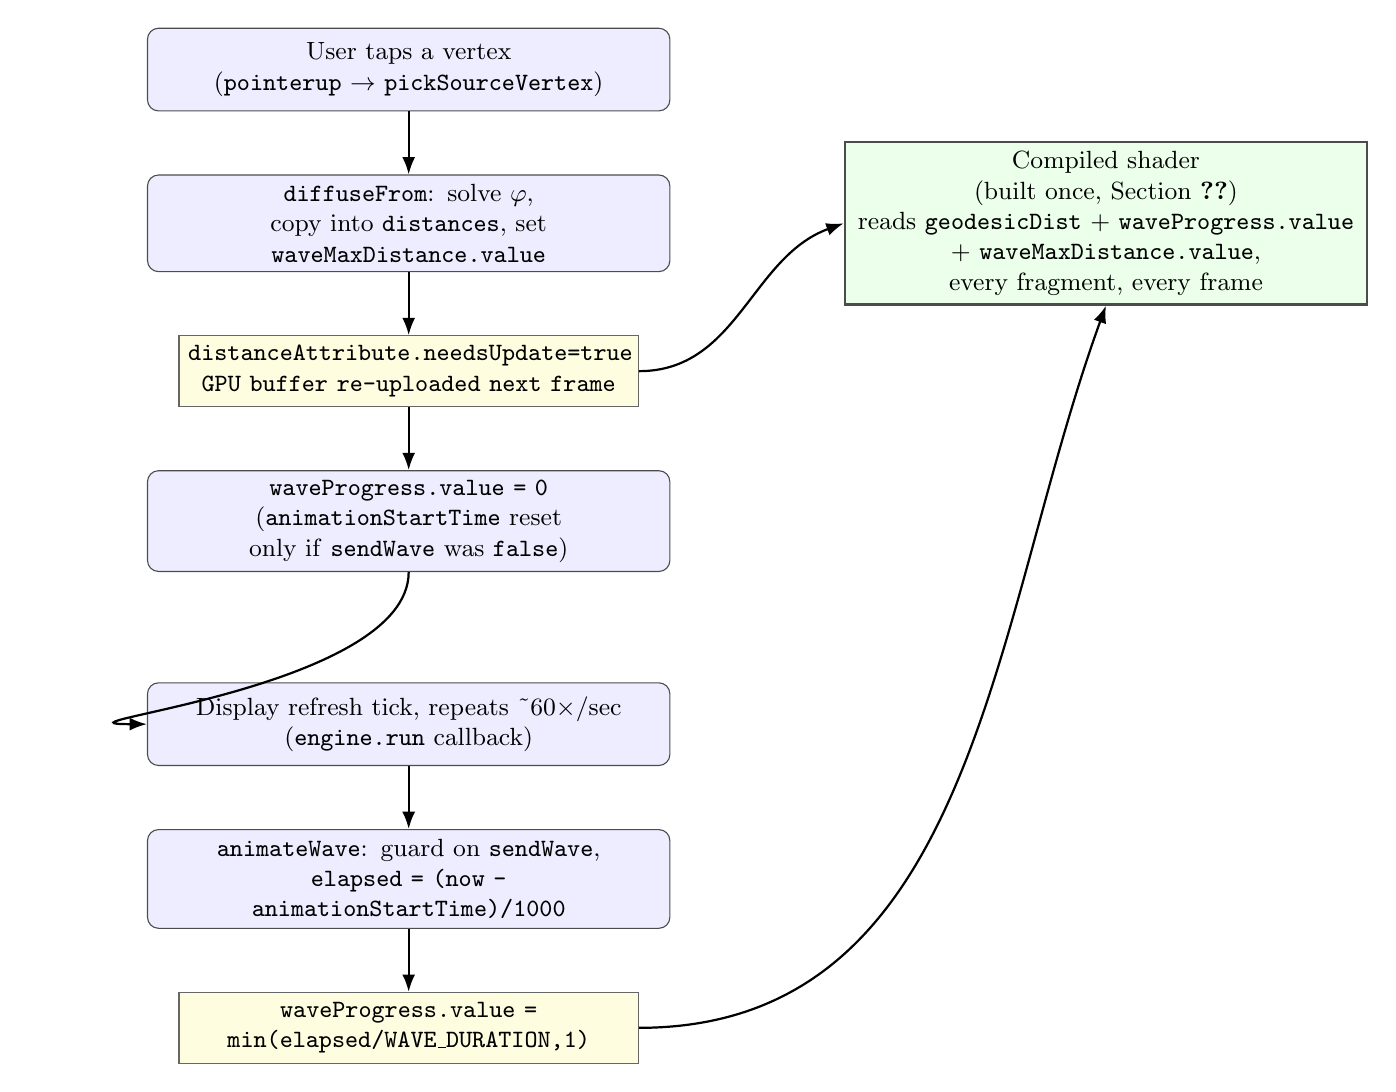
\begin{tikzpicture}[node distance=8mm]
  \node[block] (click) {User taps a vertex\\(\func{pointerup} $\to$ \func{pickSourceVertex})};
  \node[block, below=of click] (solve) {\func{diffuseFrom}: solve $\varphi$,\\copy into \code{distances}, set \code{waveMaxDistance.value}};
  \node[data, below=of solve] (upload) {\code{distanceAttribute.needsUpdate=true}\\GPU buffer re-uploaded next frame};
  \node[block, below=of upload] (reset) {\code{waveProgress.value = 0}\\(\code{animationStartTime} reset only if \code{sendWave} was \code{false})};

  \node[gpu, right=22mm of solve] (shader) {Compiled shader\\(built once, Section~\ref{sec:shader})\\reads \code{geodesicDist} + \code{waveProgress.value}\\+ \code{waveMaxDistance.value}, every fragment, every frame};

  \node[block, below=of reset, yshift=-6mm] (tick) {Display refresh tick, repeats \textasciitilde60$\times$/sec\\(\func{engine.run} callback)};
  \node[block, below=of tick] (elapsed) {\func{animateWave}: guard on \code{sendWave},\\\code{elapsed = (now - animationStartTime)/1000}};
  \node[data, below=of elapsed] (progress) {\code{waveProgress.value =}\\\code{min(elapsed/WAVE\_DURATION,1)}};

  \draw[arrowline] (click) -- (solve);
  \draw[arrowline] (solve) -- (upload);
  \draw[arrowline] (upload) -- (reset);
  \draw[arrowline] (reset.south) to[out=270,in=180] (tick.west);
  \draw[arrowline] (tick) -- (elapsed);
  \draw[arrowline] (elapsed) -- (progress);

  \draw[arrowline] (upload.east) to[out=0,in=200] (shader.west);
  \draw[arrowline] (progress.east) to[out=0,in=250] (shader.south);
\end{tikzpicture}
\end{center}

The left column (click $\to$ solve $\to$ upload $\to$ reset clock) runs once per tap. The
lower-left column (tick $\to$ elapsed $\to$ progress) runs continuously, forever, independent
of clicks. Both only ever feed \emph{data} to the single shader on the right, which itself
is built exactly once and never changes shape --- only the numbers flowing into it do. Note
that \code{waveMaxDistance.value} is written only by the left column (once per click) while
\code{waveProgress.value} is written only by the lower-left column (every frame) --- the
shader is the only place the two are ever combined.

% =====================================================================
\section{Summary: every TSL function used}
\label{sec:tslsummary}
% =====================================================================

\begin{center}
\small
\renewcommand{\arraystretch}{1.35}
\begin{tabular}{@{}p{2.7cm}p{3.6cm}p{7.1cm}@{}}
\toprule
\textbf{Function} & \textbf{GPU concept} & \textbf{Role in this file} \\
\midrule
\func{Fn(() => \{...\})} & Wraps a JS closure as one compiled, reusable node-graph
  function, rather than an inline expression. & Wraps the entire wave/color computation;
  \func{init()} calls the result once to produce \code{colorNode}. \\
\func{uniform(x)} & Uniform: one value, identical for every shader invocation, mutable from
  JS via \code{.value} without recompiling. & Backs \code{waveProgress} (per-frame) and
  \code{waveMaxDistance} (per-click) --- two independent animated inputs, not one. \\
\func{attribute(name, type)} & Attribute: one value per vertex, stored in a named GPU
  buffer; auto-promoted to an interpolated \emph{varying} when consumed per-fragment. &
  Reads the custom \code{"geodesicDist"} buffer this script wrote itself. \\
\func{float(x)} & Wraps a JS number as a graph node so it can be combined with other
  nodes. & Used for \code{roughnessNode}/\code{metalnessNode} in \func{init()}. \\
\func{a.sub(b)}, \func{a.add(b)}, \func{a.mul(b)}, \func{a.div(b)} & Graph-building
  arithmetic --- each returns a new node for the result, evaluated later on the GPU. &
  Build \code{waveCenter}, \code{normalizedDistance}, \code{i3}, and the zone offsets
  feeding each \func{mix()}. \\
\func{cos(x)} & Built-in cosine. & Produces the raised-cosine band shape
  \code{waveIntensity} --- symmetric, unlike the old one-sided \code{smoothstep} edge. \\
\func{abs(x)} & Built-in absolute value. & Used in \code{isInsideWave} to test distance
  from the band's center in either direction. \\
\func{clamp(x, lo, hi)} & Built-in range clamp. & Safety-clamps \code{finalIntensity} to
  $[0,1]$ before scaling into \code{i3}. \\
\func{a.lessThan(b)} & Comparison node --- returns a boolean-valued node, evaluated
  per-fragment. & Drives \code{isInsideWave} and the two-way zone split for the fire color
  ramp. \\
\func{a.select(ifTrue, ifFalse)} & TSL's node-graph if/else --- both branches are computed,
  the boolean picks the result per-fragment. & Masks intensity outside the band, applies
  the end-of-animation cutoff, and picks among the three fire-ramp zones (nested). \\
\func{color(hex)} & Wraps a constant RGB color as a node. & Wraps \code{BASE\_COLOR} and
  the three \code{FIRE\_COLOR} stops. \\
\func{mix(a, b, t)} & Built-in linear interpolation, $a(1{-}t)+bt$. & Used three times now
  (cyan$\to$red, red$\to$yellow, yellow$\to$white) instead of the old single
  cyan/magenta blend; assigned (via \code{waveGlowNode}) to \code{material.colorNode}. \\
\func{smoothstep(e0, e1, x)} & Built-in Hermite ($3t^2{-}2t^3$) ramp. & Still imported, but
  \textbf{no longer used} anywhere in the current shader --- vestigial from the old V1
  filled-disk version's single soft edge. \\
\bottomrule
\end{tabular}
\end{center}

% =====================================================================
\section{Future work: concurrent wave sources}
\label{sec:future}
% =====================================================================

Everything above describes a \emph{single} wave: one \code{waveProgress}/
\code{waveMaxDistance} uniform pair and one \code{geodesicDist} attribute, all overwritten
by whichever click happened most recently (with the mid-flight quirk noted in
Section~\ref{sec:oneshot}). A natural extension is letting multiple clicks spawn multiple
waves that draw on top of one another --- new ripples appearing without restarting or
interrupting ones already in flight, combined with a simple \code{max()} rather than any
real alpha/blend compositing. Three approaches were scoped, ranging from least to most
complex to integrate; none of them are implemented, and this section exists purely to
record the tradeoffs for whenever this gets picked up.

\subsection*{Option 1 --- fixed slot pool (least complex)}
Turn today's scalar state (\code{waveProgress}, \code{waveMaxDistance}, \code{distances},
\code{sendWave}, \code{animationStartTime}) into arrays of length \code{MAX\_WAVES} (e.g.\
$4$). Each click claims a slot (round-robin, evicting the oldest if all are busy), runs its
own heat-method solve into that slot's own \type{Float32Array}/\type{BufferAttribute}, and
starts its own timer. In TSL, a plain JS \code{for} loop --- unrolled at graph-build time,
since \code{MAX\_WAVES} is a compile-time constant --- builds \code{MAX\_WAVES} copies of
today's \code{waveGlowNode} math and combines them with \code{max()}.
\begin{itemize}[leftmargin=1.4em]
  \item \textbf{Pros:} Smallest possible diff --- today's single-wave logic, parameterized
    by slot index, several times over. No new GPU resource types or TSL constructs beyond
    \code{attribute()}/\code{uniform()}, already used throughout this file. Fully
    predictable memory/perf.
  \item \textbf{Cons/drawbacks:} Hard cap on concurrent waves --- a click past the limit
    must evict the oldest wave, which either vanishes abruptly mid-animation or the click
    is ignored. Each slot costs a full extra vertex attribute (cheap at this mesh's vertex
    count, but doesn't scale past a handful of slots).
\end{itemize}

\subsection*{Option 2 --- shared \code{DataTexture} (medium)}
Keep timing (\code{waveProgress}/\code{waveMaxDistance}) as a small fixed uniform array
like Option~1, but store all $N$ waves' distance fields as rows of one
\type{THREE.DataTexture} (rows = slots, columns = vertex index) instead of $N$ separate
\type{BufferAttribute}s. A click rewrites one texture row; the shader fetches a vertex's
distance for slot $i$ via a nearest-filtered texel lookup instead of \code{attribute()}.
\begin{itemize}[leftmargin=1.4em]
  \item \textbf{Pros:} Scales to a higher practical slot count before things get heavy ---
    adding a texture row is cheaper than adding a whole new vertex attribute. Consolidates
    wave storage into one resource instead of $N$ loose ones.
  \item \textbf{Cons/drawbacks:} Introduces a genuinely new pattern for this codebase:
    mapping vertex index $\to$ texture UV, and nearest-neighbor sampling must be forced or
    adjacent vertices' distances bleed into each other. Still has a fixed cap, just a
    higher one. More code than Option~1 for a benefit (bigger $N$) this demo may not
    actually need.
\end{itemize}

\subsection*{Option 3 --- dynamic storage buffer + TSL \func{Loop()} (most complex)}
Drop the cap entirely. Keep a real JS array of live waves (push on click, splice out once
\code{progress} $\ge 1$), backed by a \code{storage()} buffer sized generously (e.g.\ $64$
slots), and drive the shader with a TSL \func{Loop()} whose trip count is a \emph{uniform}
(the current active-wave count) rather than a compile-time constant --- so idle slots cost
nothing and nothing ever needs to be evicted.
\begin{itemize}[leftmargin=1.4em]
  \item \textbf{Pros:} No artificial cap and no eviction cliff --- waves fade out and their
    slot is naturally reclaimed. Shader cost tracks the actual number of concurrent waves
    per frame instead of a fixed worst case.
  \item \textbf{Cons/drawbacks:} By far the biggest jump into unfamiliar territory for this
    codebase --- storage buffers, dynamic (non-unrolled) \func{Loop()} trip counts, and
    buffer compaction as waves expire are all new, with real WebGPU footguns (buffer
    layout/alignment, upload timing). Almost certainly over-engineered for a portfolio
    piece where a handful of concurrent clicks is the realistic ceiling --- the most
    implementation risk for a payoff that may not be visually distinguishable from
    Option~1.
\end{itemize}

\end{document}
